\newpage
\section{Algoritmo de Mínimos Cuadrados}
Para implementar el algoritmo de mínimos cuadrados y poder sacar la predicción de la pendiente se desarrollaron 3 módulos en el algoritmo las cuales son:aplicación, notificación y operación.
En el módulo de \textbf{aplicación} básicamente es la estructura de la interfaz de la aplicación, el módulo de \textbf{notificación} manda el mensaje junto con la imagen de la gráfica resultante del algoritmo y por último el módulo de \textbf{operación} es en sí todo el desarrollo del algoritmo de mínimos cuadrados.

\begin{itemize}
\item \textbf{Aplicación}
Empieza por la adquisición de información como se puede ver en la siguiente imagen         \ref{image:1}

\FloatBarrier
\begin{figure}[htbp!]
		\centering
		    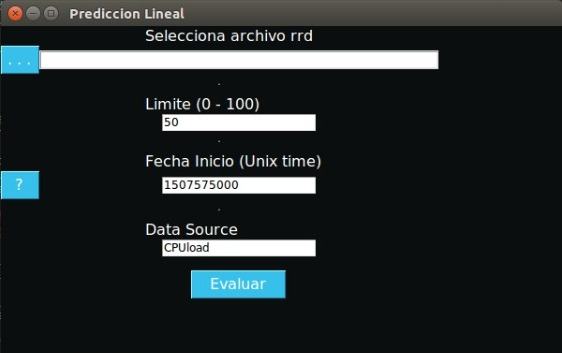
\includegraphics[width=.6 \textwidth]{../images/1.jpeg}
		\caption{Inicio de la interfaz de mínimos cuadrados.}
		\label{image:1}
\end{figure}
\FloatBarrier

La petición de datos implica:
1. La base de datos RRD con la que se va a trabajar el algoritmo de predicción.
2. El límite superior, en donde ese valor se intersecta con la recta definida con el algoritmo de predicción.
3. La fecha de inicio, a partir de este valor, comenzará a evaluar nuestro algoritmo, no será necesario introducir la fecha de la última actualización porque nuestro algoritmo lo puede resolver, dicho método se explicará posteriormente.
4. Data Source, es la variable en donde la base de datos comenzará a recuperar información, será importante para generar la gráfica y asociar el algoritmo de predicción con dicha variable.

\FloatBarrier
\begin{figure}[htbp!]
		\centering
		    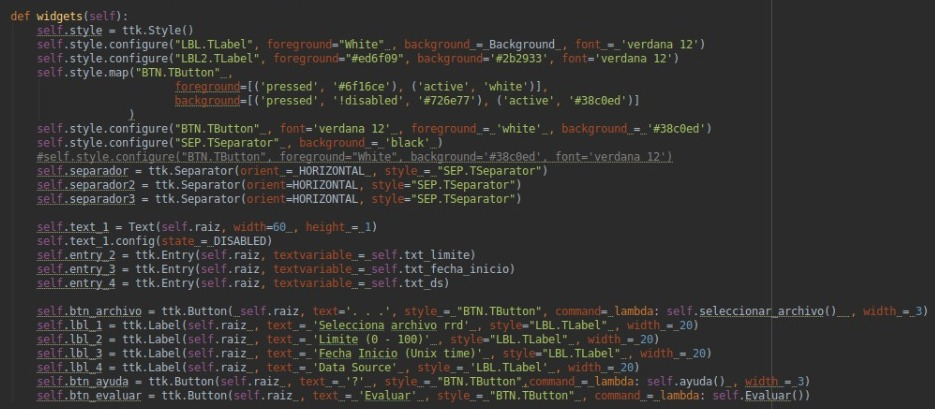
\includegraphics[width=1 \textwidth]{../images/ap2.jpeg}
		\caption{Ingreso de valores.}
		\label{image:ap2}
\end{figure}
\FloatBarrier

Se hacen las validaciones pertinentes como se muestra en la imagen \ref{image:ap1} para que no haya ningún campo sin llenar, tanto la ruta del archivo como los valores deben ser ingresados o por su defecto son los valores, que se tienen por default.
En la línea 85 se evalúa la hora estimada en la que se pronostica que el fallo podrá ocurrir, en determinada forma es la función más importante ya que en ella se evalúa el método de mínimos cuadrados y se regresa el valor en tiempo UNIX, como conclusión tenemos ese valor en la variable ``estimado".

En la línea 86 se manda llamar la función que nos generará la gráfica con los valores, enviando así mismo la hora estimada para que pueda trazar una línea vertical representando con mayor precisión la hora de la predicción del fallo.

Si la respuesta es Error, quiere decir que ha ocurrido un error al momento de graficar
\FloatBarrier
\begin{figure}[htbp!]
		\centering
		    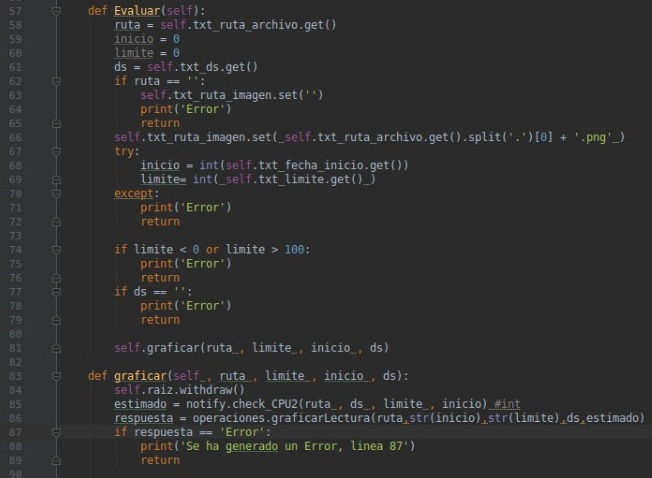
\includegraphics[width=.7 \textwidth]{../images/ap1.jpeg}
		\caption{Validación de campos de datos.}
		\label{image:ap1}
\end{figure}
\FloatBarrier

Posteriormente sigue el código como se ve en la imagen \ref{image:ap3} que presenta la información, que consta de:
Una variable llamada \textbf{strinicio} declarada en la línea 96 la cual nos va a imprimir en Una etiqueta la fecha en la que se comenzó a evaluar los valores de la base de datos.

Una variable llamada \textbf{strfin} la cual determina en que momento se tomó el último valor en la base de datos.

Una variable llamada \textbf{strpred} el cual representa la hora exacta en la que el fallo está pronosticado, este valor lo tomamos de la variable ``estimado".

Finalmente una imagen la cual fué generada en la función: \textbf{graficarLectura} de la línea 86.

\FloatBarrier
\begin{figure}[htbp!]
		\centering
		    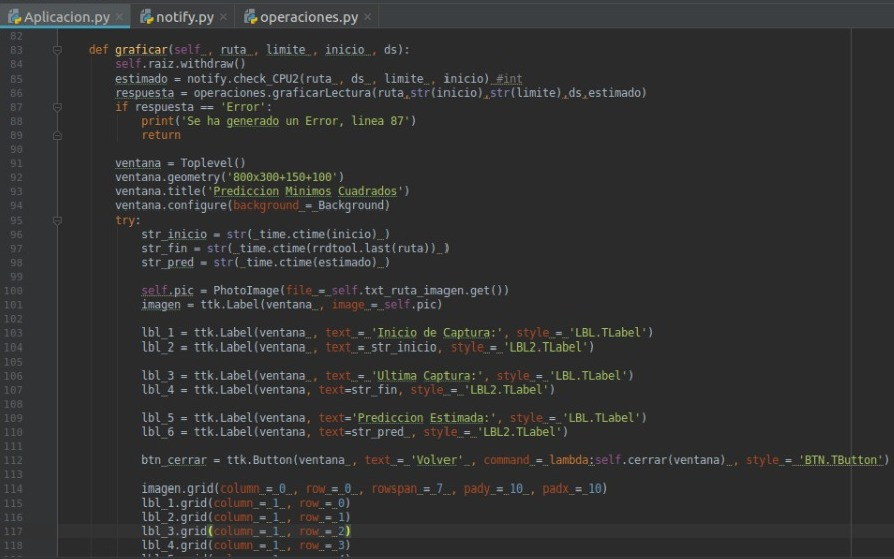
\includegraphics[width=.9 \textwidth]{../images/ap3.jpeg}
		\caption{Función graficar.}
		\label{image:ap3}
\end{figure}
\FloatBarrier


\item \textbf{Notificación}

La función \textbf{CPU} es la más importante ya que al final del proceso regresará la fecha en tiempo UNIX de la predicción que queremos realizar, dicho de otro modo, al registrar los valores de carga de CPU queremos saber, por ejemplo, en qué momento llegará esa carga al 60 por ciento, entonces para solucionar este problema se implementa el algoritmo de mínimos cuadrados, el cual es utilizado de la siguiente manera:

Declaramos la variable info para saber cada cuanto tiempo se realiza un step en la base de datos, ese valor se almacena en la variable rrdstep.
La variable estimado tendrá el valor final en el que la predicción coincide con el porcentaje de carga de CPU al que queremos evaluar. Inicialmente comienza desde la fecha de inicio de captura de datos más el step que sería equivalente a la primer captura.

Posteriormente declaramos un nombre para un archivo temporal ya que no queremos que por el momento nos genere una gráfica, más bien, queremos aprovechar las bondades de la función graph para poder realizar el algoritmo de mínimos cuadrados.

Posteriormente viene un while infinito, se detendrá hasta que la predicción supere el 100 por ciento o encuentre el valor que estamos buscando.

Realizamos el método graph en el que como inicio se declara el inicio de la captura de datos de la base RRD, como fecha final se coloca el valor estimado, tiene la finalidad de que en ese rango que será variable, evalúe mínimos cuadrados y el valor final compararlo con el valor que esperamos obtener.

El algoritmo se realiza de la siguiente manera, tomando en cuenta que la predicción de mínimos cuadrados se basa en la recta \textbf{y = mx + b:}
definimos la variable carga la cual tendrá la colección de datos de la carga de CPU desde el inicio hasta el valor estimado que en primera instancia solo es de un step.
La variable a utiliza la función \textbf{LSLSLOPE} que representa la pendiente de la recta (m) utilizando la colección de valores.
La variable b utiliza la función \textbf{LSLINT} que representa la ordenada al origen (b).Avg2 realiza el algoritmo de obtención del valor Y, lo que hace es extraer los valores de carga con un POP, tiene la variable y los multiplica, teniendo así: mx de la ecuación inicial.
Posteriormente le suma b, teniendo así \textbf{mx + b}, como resultado tenemos el valor en Y de ese rango de valores.

Realizamos la función PRINT para poder recuperar el último valor del algoritmo. Entonces en conclusión cada iteración se evalúa a un tiempo estimado la última evaluación del método de mínimos cuadrados, por lo que de obtener el valor esperado tendremos también la fecha esperada y será el valor de retorno.

Dentro del bloque try realizamos un cast del último valor capturado en el método de mínimos cuadrados y evaluamos que si es mayor o igual al valor que esperamos nos regrese la fecha estimada, si no es así, si el valor es mayor a 100 encontramos un error y regresar la última fecha de captura de información.

Si ninguno de estos casos se cumple, entonces aumentamos nuestra variable estimado en un step más. Por tanto recorremos a cada paso el algoritmo hasta encontrar nuestro valor esperado.
Se pueden ver en las imágenes \ref{image:not1} y \ref{image:not2} 

\FloatBarrier
\begin{figure}[htbp!]
		\centering
		    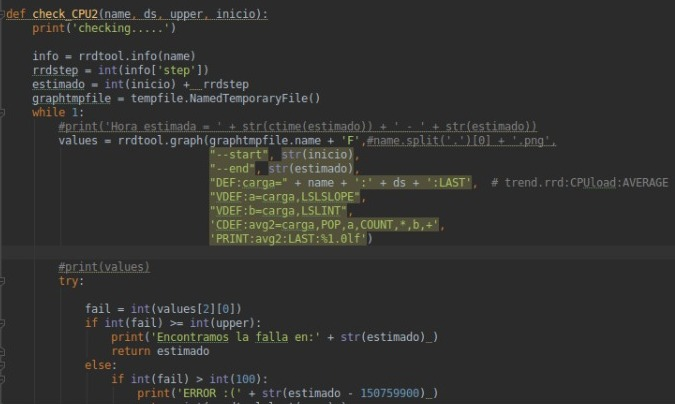
\includegraphics[width=.8 \textwidth]{../images/not1.jpeg}
		\caption{Función checkCPU.}
		\label{image:not1}
\end{figure}
\FloatBarrier

\FloatBarrier
\begin{figure}[htbp!]
		\centering
		    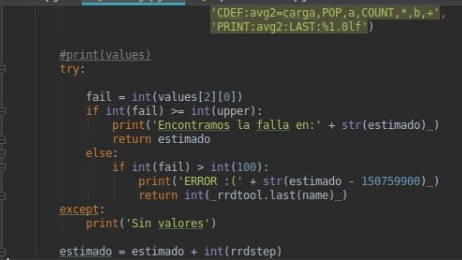
\includegraphics[width=.6 \textwidth]{../images/not2.jpeg}
		\caption{Validación de la función checkCPU.}
		\label{image:not2}
\end{figure}
\FloatBarrier

\item \textbf{Operación}

La función \textbf{GraficarLectura} recibe 5 parámetros los cuales son:
1) el nombre de la base de datos
2) la hora de inicio de captura de datos
3) el límite en donde se realizará la estimación en porcentaje, por ejemplo, 60 por ciento de la carga de CPU
4) el data source de la base de datos
5) la fecha en tiempo UNIX que el algoritmo de predicción regresó

Se ocupa la función \textbf{graph} de rrdtool la cual indica:
el nombre del archivo que va a generar, en este caso es una imagen png.
la fecha de inicio y final en la cual graficará, que la hora final se especificó 10 minutos después del fallo para poder apreciar bien la línea que marca la intersección con el fallo.
Definimos los límites y una variable llamada carga que obtiene una lista con los últimos valores capturados en la base de datos a través del tiempo.
Posteriormente, se declara una línea horizontal con el valor establecido con el cual queremos realizar la predicción.
Realizamos el algoritmo de mínimos Cuadrados con el fin de poder apreciar la línea recta que genera.
Finalmente se utiliza \textbf{VRULE} para trazar una línea vertical en una fecha específica, esta línea representa el fallo que se calculó previamente, por lo que el resultado final imprime una línea vertical a la hora del posible próximo fallo con el fin de apreciarlo gráficamente.

Si todo el proceso salió bien regresa \textbf{'Exito'}, de lo contrario regresa \textbf{'Error'}.
El código se puede ver en la imagen \ref{image:op1}

\FloatBarrier
\begin{figure}[htbp!]
		\centering
		    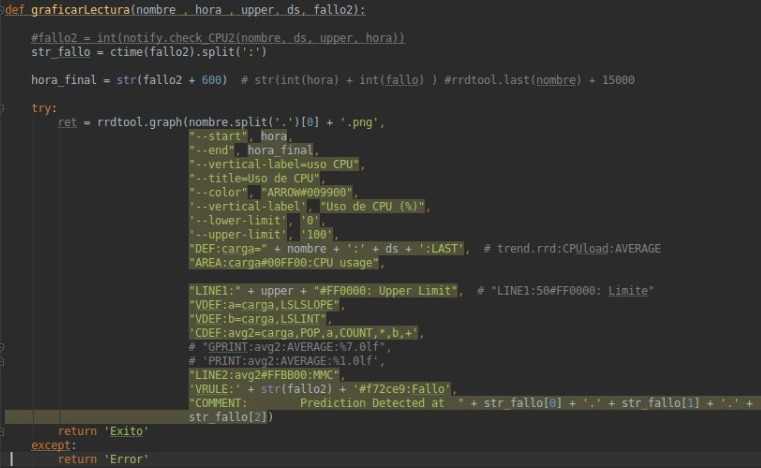
\includegraphics[width=.9 \textwidth]{../images/op1.jpeg}
		\caption{Función graficar.}
		\label{image:op1}
\end{figure}
\FloatBarrier

\end{itemize}

Finalmente el ejercicio a desarrollar en la práctica 2 se trato de sacar la recta de predicción de mínimos cuadrado con base a los datos obtenidos en el archivo \textbf{source3.rdd} con un límite de umbral de un \textbf{90}  y la fecha de inicio \textbf{1539659123} la cual esta en formato Unix y por último el archivo data source \textbf{CPUload} como se muestra en la imagen  \ref{image:inicio}

\FloatBarrier
\begin{figure}[htbp!]
		\centering
		    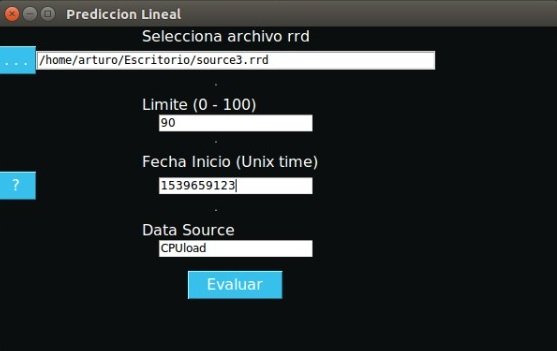
\includegraphics[width=.7 \textwidth]{../images/inicio.jpeg}
		\caption{Valores para iniciar la grafica de Mínimos cuadrados.}
		\label{image:inicio}
\end{figure}
\FloatBarrier

Como resultado de los valores ingresados se obtuvo la siguiente gráfica que nos calcula el momento exacto en donde la predicción de mínimos cuadrados rebasa el umbral dándonos el día y hora de dicho cruce.

\FloatBarrier
\begin{figure}[htbp!]
		\centering
		    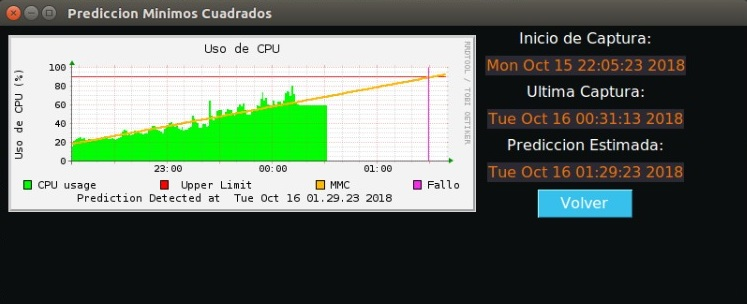
\includegraphics[width=.9 \textwidth]{../images/graficar.jpeg}
		\caption{Grafíca resultante del algoritmo de mínimos cuadrados.}
		\label{image:graficar}
\end{figure}
\FloatBarrier

Nos da como resultado el dia \textbf{ jueves 16 de octubre del 2018 a la 1:29:23 hrs.}